% ================================================================
%  DSC 208R -- Data Management for Analytics
%  Cloud Computing (Part 1): Comprehensive Review
%  Source: "Data Engineering for ML -- Cloud Computing Part 1"
% ================================================================
\documentclass[11pt]{article}

% -------------------- Packages --------------------
\usepackage[utf8]{inputenc}
\usepackage{amsmath,amssymb,amsfonts}
\usepackage{graphicx}
\usepackage{booktabs}
\usepackage{tikz}
\usetikzlibrary{positioning}
\usepackage{enumitem}
\usepackage{hyperref}
\usepackage{caption}
% -------------------- Packages --------------------
\usepackage[utf8]{inputenc}
\usepackage{amsmath,amssymb,amsfonts}
\usepackage{graphicx}
\usepackage{booktabs}
\usepackage{tikz}
\usetikzlibrary{positioning}
\usepackage{pgfplots}
\usepackage{enumitem}
\usepackage{listings}
\usepackage{hyperref}
\usepackage{caption}
\pgfplotsset{compat=1.17}

% -------------------- Listings --------------------
\lstset{
  basicstyle=\ttfamily\small,
  keywordstyle=\bfseries,
  commentstyle=\itshape,
  showstringspaces=false,
  frame=single,
  breaklines=true
}

% -------------------- Document --------------------
\begin{document}

\begin{center}
  {\LARGE\bfseries Cloud Computing -- Part 1}\\[2mm]
  {\large Comprehensive Review}\\[1mm]
  {\normalsize DSC 208R -- Parallel Data Processing and the Cloud}
\end{center}
\vspace{-0.6em}\hrule\vspace{0.9em}

\tableofcontents
\newpage

% ================================================================
\section{Motivation}

Cloud computing rents compute, storage, memory, and networking resources from remote servers.  
Key advantages over on-premise clusters are

\begin{itemize}[itemsep=0pt]
  \item \textbf{Manageability}: hardware is the provider’s problem.
  \item \textbf{Pay as you go}: fine-grained pricing from seconds to years.
  \item \textbf{Elasticity}: capacity can grow or shrink with workload demand.
\end{itemize}
These points frame the appeal of Infrastructure as a Service (IaaS), Platform as a Service (PaaS), and Software as a Service (SaaS).:contentReference[oaicite:0]{index=0}

% ================================================================
\section{Layered Model of Cloud Services}

\begin{table}[h]
\centering
\caption{Typical cloud layers and AWS examples.}
\begin{tabular}{@{}lll@{}}
\toprule
Layer & User control & Example AWS services\\
\midrule
IaaS & OS, runtime, data & EC2, EBS, VPC, S3\\
PaaS & Code, data        & Aurora, Redshift, EMR, DynamoDB\\
SaaS & Only usage       & SageMaker, Textract, Chime\\
\bottomrule
\end{tabular}
\end{table}

From a renter’s view, control decreases as one moves from IaaS to SaaS, while management burden also decreases.:contentReference[oaicite:1]{index=1}

% ================================================================
\section{Evolution of Cloud Infrastructure}

\begin{enumerate}[itemsep=0pt]
  \item \textbf{Cloud 1.0}: networked servers; users rent whole machines.
  \item \textbf{Cloud 2.0}: virtualized servers and multi-tenancy; users rent resource \emph{capacity}, enabling load balancing and better elasticity.
  \item \textbf{Cloud 3.0} (ongoing): serverless and fully disaggregated resources connected by fast networks.
\end{enumerate}
Each generation gives the provider more flexibility to pack workloads efficiently.:contentReference[oaicite:2]{index=2}

% ================================================================
\section{Parallelism Paradigms Revisited}

Traditional parallel styles carry into the cloud:

\begin{itemize}[itemsep=0pt]
  \item \textbf{Shared-nothing}: independent workers with local data (dominant in RDBMS, Hadoop, Spark).
  \item \textbf{Shared-memory}: nodes share a large memory space.
  \item \textbf{Shared-disk}: nodes share a storage layer (now common via S3 plus local EBS).
\end{itemize}

Modern data-center networks hit 100 Gbps or more, making hybrids common: compute on EC2, data on S3 (shared-disk), and local shuffles in EBS (shared-nothing).:contentReference[oaicite:3]{index=3}

% ================================================================
\section{Example IaaS Architecture on AWS}

\begin{figure}[h]
  \centering
  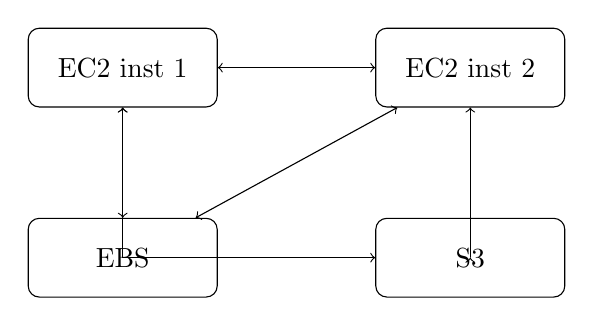
\begin{tikzpicture}[
    node/.style={draw,rounded corners,minimum width=2.4cm,minimum height=1cm},
    yshift=-0.2cm
  ]
    \node[node] (ec2a) {EC2 inst 1};
    \node[node,right=2.0cm of ec2a] (ec2b) {EC2 inst 2};
    \node[node,below=1.4cm of ec2a] (ebs)  {EBS};
    \node[node,below=1.4cm of ec2b] (s3)   {S3};

    \draw[<->] (ec2a) -- (ec2b);
    \draw[<->] (ec2a) -- (ebs);
    \draw[<->] (ec2b) -- (ebs);
    \draw[<->] (ec2a.south) |- (s3);
    \draw[<->] (ec2b.south) |- (s3);
  \end{tikzpicture}
  \caption{Shared-nothing compute with shared-disk storage in AWS.}
\end{figure}

% ================================================================
\section{New Renting Paradigms}

\subsection{Spot vs On-Demand Instances}

\begin{itemize}[itemsep=0pt]
  \item \textbf{On-Demand}: fixed hourly price, no interruption risk.
  \item \textbf{Spot}: bid for unused capacity; price fluctuates, instance can be reclaimed with short notice.
\end{itemize}

Spot can cut costs by up to an order of magnitude but suits only fault-tolerant or checkpointed jobs.:contentReference[oaicite:4]{index=4}

\subsection{Serverless Function as a Service}

Users upload a function and pay for milliseconds of execution time; the provider scales instances automatically.  This model embodies Cloud 3.0’s disaggregated compute vision.

% ================================================================
\section{Pros and Cons Summary}

\begin{itemize}[itemsep=0pt]
  \item \textbf{Pros}
    \begin{itemize}[itemsep=0pt]
      \item No hardware maintenance.
      \item Fine-grained cost aligned with usage.
      \item Rapid elasticity to meet workload spikes.
    \end{itemize}
  \item \textbf{Cons}
    \begin{itemize}[itemsep=0pt]
      \item API and licensing complexity; need CloudOps skills.
      \item Long-term spend can exceed on-premise clusters.
      \item Vendor lock-in, outage, and security concerns.
    \end{itemize}
\end{itemize}

% ================================================================
\section{Future Directions}

\begin{itemize}[itemsep=0pt]
  \item Fully disaggregated resources with sub-second elasticity.
  \item Cross-vendor orchestration to mitigate lock-in.
  \item Better cost observability and automated budget guards.
\end{itemize}

% ================================================================
\section*{Conclusion}

Cloud Computing Part 1 highlights why elastic, pay-as-you-go resources have reshaped data analytics.  
Understanding service layers, evolving infrastructure, and new renting paradigms equips practitioners to balance cost, performance, and operational risk in modern data pipelines.:contentReference[oaicite:5]{index=5}

\end{document}
